\chapter{Eurocopter AS350}
\label{ch:Eurocopter AS350}

\emph{This chapter opens with an introduction to the helicopter named Eurocopter AS350, its development over the years and some technical features. In follow deals with the study of the tail in particular \dots, where the aeroelastic problem will be neglected and as a result all the aerodynamic components will be removed from the model.}

\section{Introduction}
The \textbf{Eurocopter AS350 Écureuil} (\emph{Squirrel}) is a single-engine light helicopter originally designed and manufactured in France by Aérospatiale, now Airbus Helicopters. In North America, the AS350 is marketed as the AStar. The AS355 Ecureuil 2 is a twin-engine variant, marketed in North America as the TwinStar. The Eurocopter EC130 is a derivative of the AS350 airframe and is considered by the manufacturer to be part of the Écureuil single-engine family.
In the early 1970s, Aérospatiale decided to initiate a new development programme to produce a suitable replacement for the aging Aérospatiale Alouette II.
While the Aérospatiale Gazelle, which had been developed in the 1960s and 1970s, had been met with numerous orders by military customers, commercial sales of the type had been less than anticipated, thus the need for a new civil-orientated development was identified.
The development of the new rotorcraft, which was headed by Chief Engineer René Mouille, was focused on the production of an economic and cost-effective aerial vehicle, thus both Aérospatiale's Production and Procurement departments were heavily involved in the design process.
One such measure was the use of a rolled sheet structure, a manufacturing technique adapted from the automotive industry; another innovation was the newly developed Starflex main rotor. It was also decided that both civil and military variants of the emergent helicopter would be developed to conform with established military requirements\cite{wiki:xxx}.

\begin{minipage}{\textwidth}
  \begin{minipage}[b]{0.49\textwidth}
   	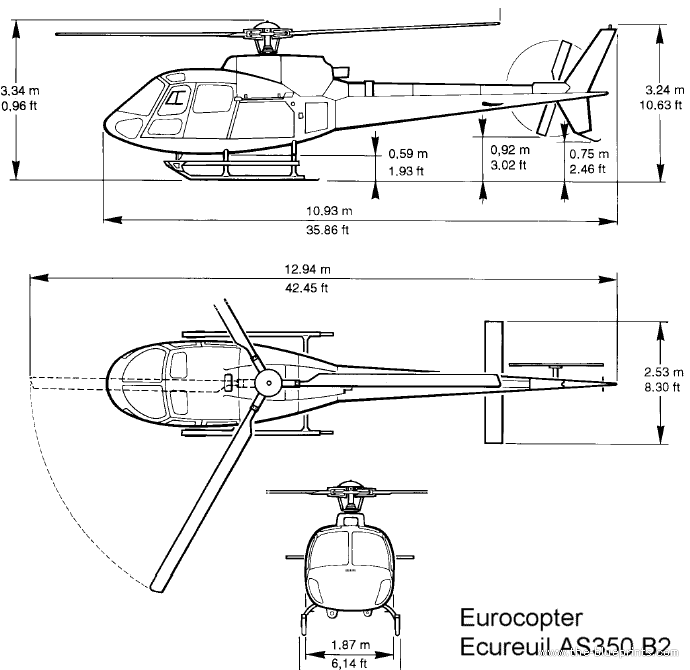
\includegraphics[width=\textwidth]{eurocopter-as350-b2}
    \captionof{figure}{AS350 blueprints\label{fig:AS350blueprints}}
  \end{minipage}
  \hfill
  \begin{minipage}[b]{0.49\textwidth}
    \centering
    \begin{tabular}{%
		>{}l%
		>{}l%
		>{\columncolor{yellow}}r}
		\multicolumn{2}{>{\columncolor{lightgray}}c}{General characteristics}\\
		Length	&	12.94 m\\
		Height	&	3.34 m\\
		Main rotor diameter& 10.69 m\\
		Empty weight		& 1220 kg\\
		Max takeoff weight & 2250 kg\\
		capability	& 2500 kg\\
		\multicolumn{2}{>{\columncolor{lightgray}}c}{Propulsion}\\
		Powerplant	&	1 x Turbine\\ 
		& Turbomeca\\& Arriel 1D1\\
		Power	&	546 kW\\
		\multicolumn{2}{>{\columncolor{lightgray}}c}{Performance}\\
		Maximum speed & 287 km/h\\
		Range	 & 476 km\\
		service ceiling 	 & 6100 m\\
    \end{tabular}
  \captionof{table}{Main characteristics AS350}\end{minipage}
\end{minipage}

\begin{figure}[t]
\centering
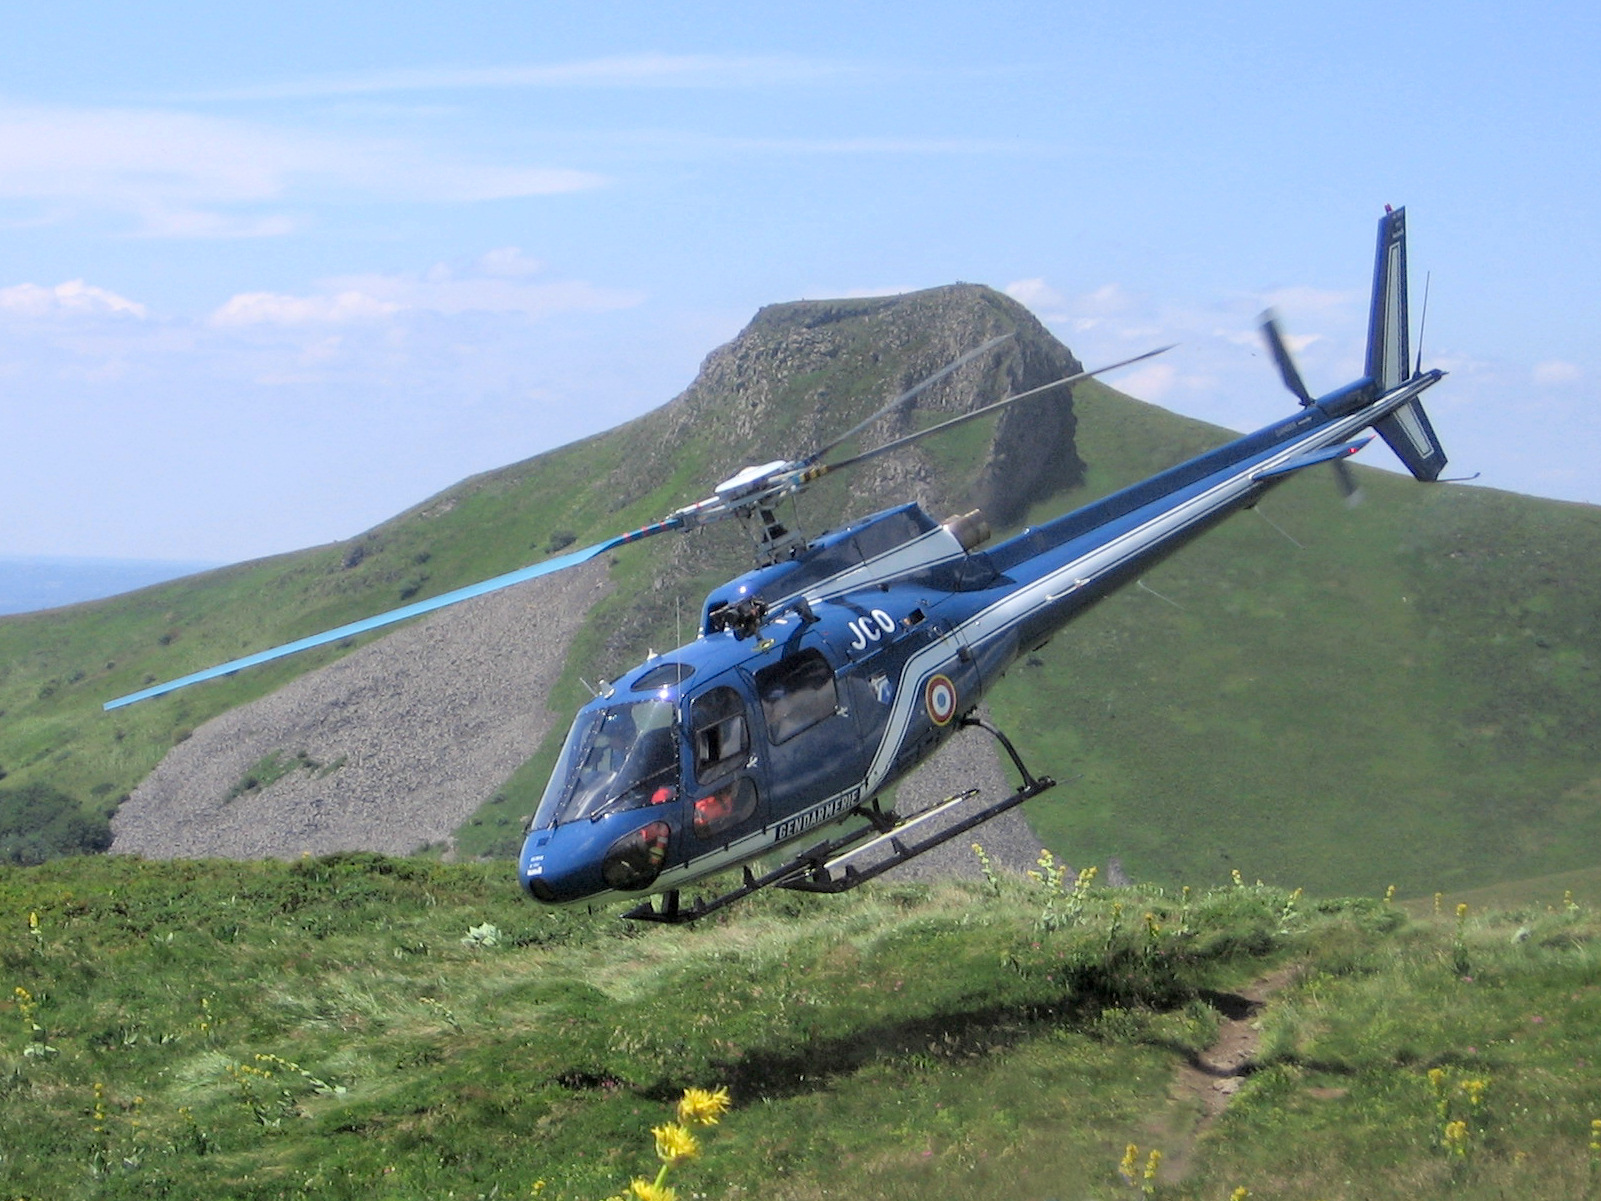
\includegraphics[width=0.80\textwidth]{Helicopter_rescue_sancy_takeoff}
\caption{Helicopter takeoff \\Di Fabien1309 - Own work}
\label{fig:AS350wiki}
\end{figure}

\section{Geometric model}
The geometric model is shared among three different configuration where was enfatizated a different approach to evalute the repsonce of structural elemtents in different condition of approximation. Infact the first case is an evalution of the simple model where considering only tail like as a cantilever beam. 
While in the second case considering also the trasmission shaft rigidly linked at the tail and the presence of a lumped mass to simulate the persence of the block of rotor in the proximity the end of tail. 
Finally consider a third model where we considering the shaft's weight is distributed along the lenght of tail like as lumped mass, we consider as before another concentrated mass to represent the block of rotor at the tail's end.
The model was obtained by the revolution of seven contiguous segments with respect to axis placed in the plane $xz$, thus obtaining a truncated cone having a radius $325\,mm$ at the base and a radius $50\,mm$ for the minor base, the whole extension is $5.2\,m$.
The cone trunk was highlighted in twentyfour equal segments in order to obtain a bse for the reallization of components such as stringer, horizontal stabilizer attachment, stiffners and ribs.
The result can be seen in the figure \ref{fig:Ansys1}.

\begin{figure}[htb]
\centering
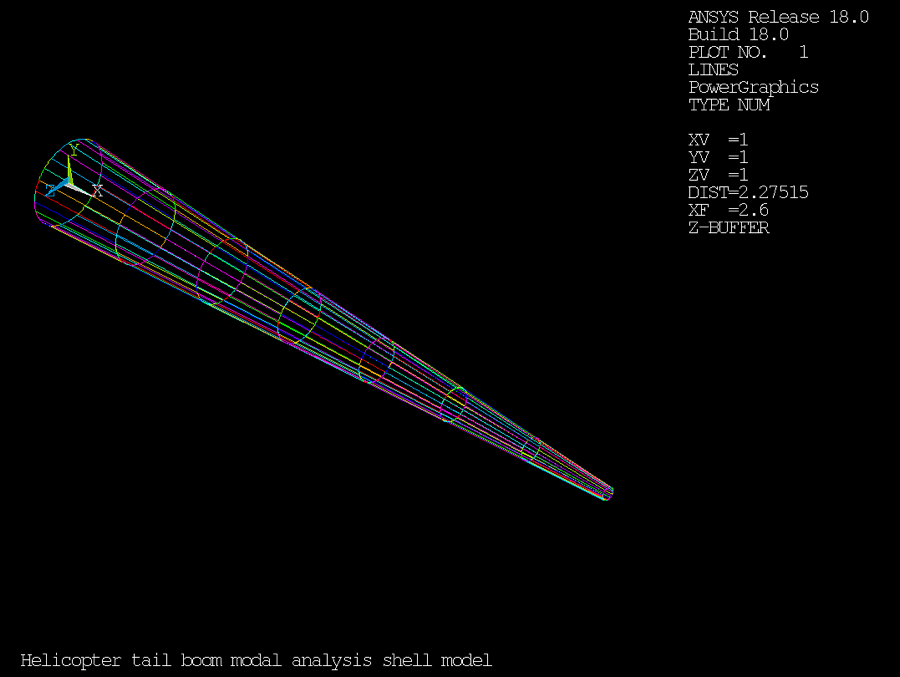
\includegraphics[width=0.8\textwidth]{/ShellModel/Shellmodel000}
\caption{AS350 ansys model}
\label{fig:Ansys1}
\end{figure}

\section{Mesh model}
After the geometric model has been realized, the finite element model has the same types of shared elements to ensure consistency between the models, as well as the texture of the matrices used to study the different models.
\subsection{Simple model}
For structural elements such as:
\begin{itemize}
\item stringer;
\item horizontal stabilizer attachment;
\item stiffners;
\item ribs.
\end{itemize}
Type elements have been used: \textsc{beam189}, this type of element has been assigned a rectangular section and a square as shown in \ref{fig:SectionGeometry}. Specifically, the rectangular section, fig. \ref{subfig:Rectagnle}, is intended to form the stinger and longerons components, instead the square section, fig.\ref{subfig:Square}, perform the ribs, then the structure skeleton are represented in fig. \ref{fig:Ansys1Mesh}.

The material used is steel with the following properties:
\begin{itemize}
\item Young's modulus, $205\,[GPa]$ 
\item Poisson's ratio, $0.29$
\item Density, $7850	\,[kg/m^3]$
\end{itemize}

\begin{figure}[!htb]
\centering
\subfloat[][\emph{Rectangular}.\label{subfig:Rectagnle}]{
   \resizebox{.25\linewidth}{!}{\begin{tikzpicture}
%linee guida
%\foreach \x in {0,1,...,15}
%   \draw [help lines] (\x,0) node [below,%
%          font=\footnotesize] {$\x$} -- (\x,15);
%%\foreach \y in {0,1,...,15}
%%   \draw [help lines] (0,\y) node [left,%
%%          font=\footnotesize] {$\y$} -- (15,\y);

\node at (1,14) (a) {};
\node at (3,14) (b) {};
\node at (3,10) (c) {};
\node at (1,10) (d) {};

\draw (a) rectangle (c);
\draw[-latex] (2,12)--( 2,9.5)node[right]{\scriptsize x};
\draw[-latex] (2,12)--(3.5,12)node[above]{\scriptsize y};


% quote track
 \dimline    [color=gray,
 			  label style={above=0.1ex},
                % line style={thick},
                %extension start style={gray,thin},
                %extension end style={gray,thin},
                extension start length=0.5cm,
                extension end length=0.5cm
                ]{(1,14.5)}{(3,14.5)}{$b$};
                
\dimline    [color=gray,
                % line style={thick},
                %extension start style={gray,thin},
                %extension end style={gray,thin},
                extension start length=0.5cm,
                extension end length=0.5cm
                ]{(0.5,10)}{(0.5,14)}{$w$};
\end{tikzpicture}}} \quad
\subfloat[][\emph{Square}.\label{subfig:Square}]{
   \resizebox{.25\linewidth}{!}{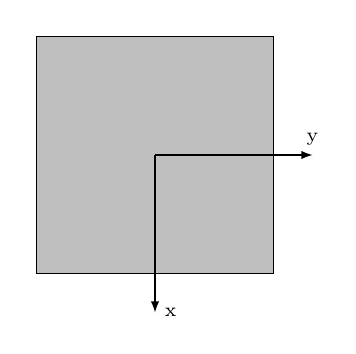
\begin{tikzpicture}
%linee guida
%\foreach \x in {0,1,...,15}
%   \draw [help lines] (\x,0) node [below,%
%          font=\footnotesize] {$\x$} -- (\x,15);
%\foreach \y in {0,1,...,15}
%   \draw [help lines] (0,\y) node [left,%
%          font=\footnotesize] {$\y$} -- (15,\y);

\node at (1,14) (a) {};
\node at (4,14) (b) {};
\node at (4,11) (c) {};
\node at (1,11) (d) {};

\draw[fill=lightgray] (a) rectangle (c);
\draw[-latex] (2.5,12.5)--( 2.5,10.5)node[right]{\scriptsize x};
\draw[-latex] (2.5,12.5)--(4.5,12.5)node[above]{\scriptsize y};


% quote track
 \dimline    [color=gray,
 			  label style={above=0.1ex},
                % line style={thick},
                %extension start style={gray,thin},
                %extension end style={gray,thin},
                extension start length=0.5cm,
                extension end length=0.5cm
                ]{(1,14.5)}{(4,14.5)}{$5$};
                
\dimline    [color=gray,
			label style={above=0.1ex},
                % line style={thick},
                %extension start style={gray,thin},
                %extension end style={gray,thin},
                extension start length=0.5cm,
                extension end length=0.5cm
                ]{(0.5,11)}{(0.5,14)}{$5$};
\end{tikzpicture}}}\\
\caption{Section for element \textsc{beam189}}
\label{fig:SectionGeometry}
\end{figure}

\begin{figure}[!htb]
\centering
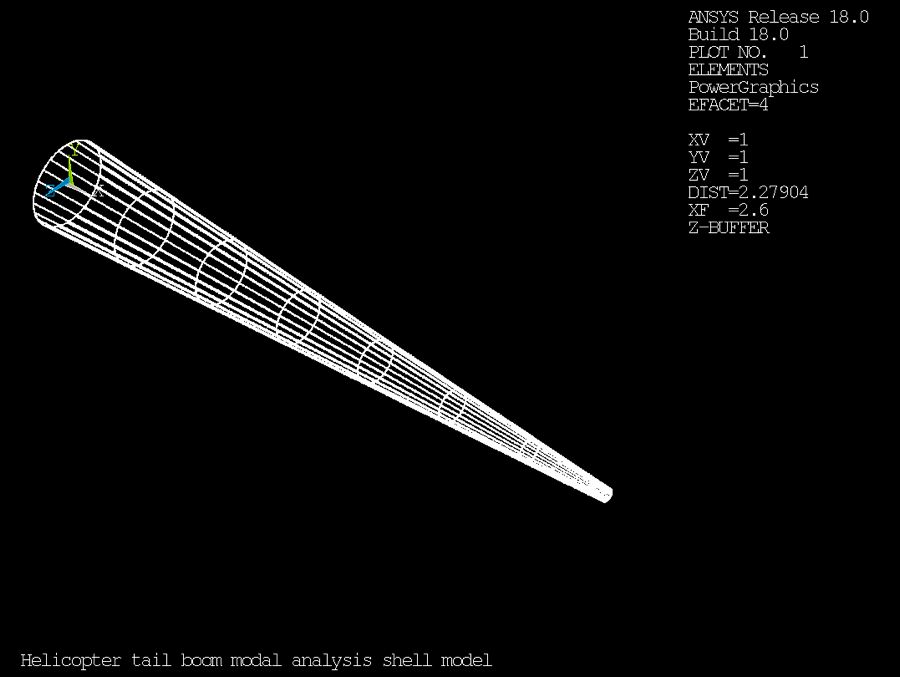
\includegraphics[width=0.8\textwidth]{/ShellModel/Shellmodel001}
\caption{Skeleton mesh model}
\label{fig:Ansys1Mesh}
\end{figure}

\noindent On the other hand, to realize the mantle covering the support structure was used type element: \textsc{shell181} with aluminum used as material with the following properties:
\begin{itemize}
\item Young's modulus: $64\,[GPa]$;
\item Poisson's ratio: $0.34$;
\item Density: $2700\,[kg/m^3]$.
\end{itemize}
Finally, you can see the full model in the figure \ref{fig:Ansys2Mesh}.

\begin{figure}[!htb]
\centering
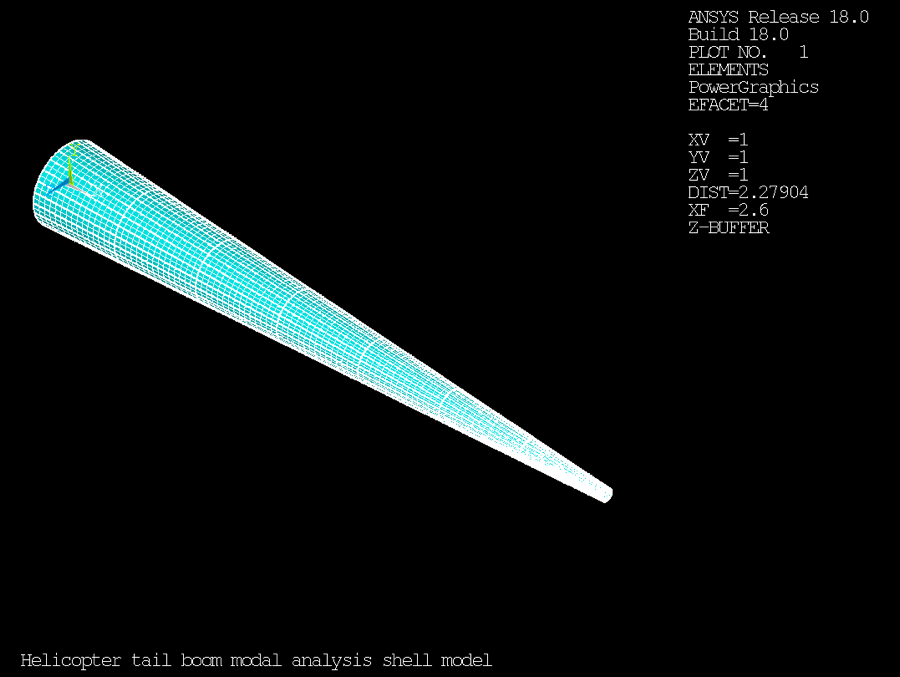
\includegraphics[width=0.8\textwidth]{/ShellModel/Shellmodel002}
\caption{Complete mesh model}
\label{fig:Ansys2Mesh}
\end{figure}

\subsection{Simple model with shaft}
In this case, the geometric model has the same features as the previously described model, with the addition of a transmission shaft on top of the cone.
the shaft has been modellated with type of elements \textsc{beam189} with tube section, fig. \ref{fig:SectCTube}, and realized in duralumin characterized by the following property:
\newpage
\begin{itemize}
\item Young's modulus: $72\,[GPa]$;
\item Poisson's ratio: $0.33$;
\item Density: $2810\,[kg/m^3]$.
\end{itemize}

\begin{figure}[!htb]
\centering
\resizebox{.25\linewidth}{!}{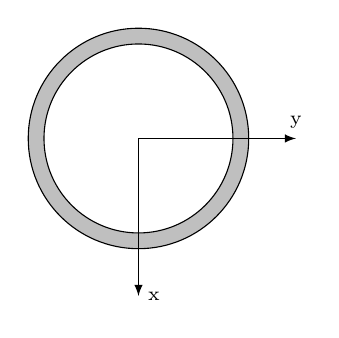
\begin{tikzpicture}
%linee guida
%\foreach \x in {0,1,...,15}
%   \draw [help lines] (\x,0) node [below,%
%          font=\footnotesize] {$\x$} -- (\x,15);
%\foreach \y in {0,1,...,15}
%   \draw [help lines] (0,\y) node [left,%
%          font=\footnotesize] {$\y$} -- (15,\y);

% InternalRadius, 0.012
% ExternalRadius, 0.014
\draw[fill=lightgray] (7.5,7.5) circle (14mm);
\draw[fill=white] (7.5,7.5) circle (12mm);
%reference system
\draw[-latex] (7.5,7.5)--(7.5,5.5)node[right]{\scriptsize x};
\draw[-latex] (7.5,7.5)--(9.5,7.5)node[above]{\scriptsize y};

%% quote track
 \dimline    [color=gray,
 			  label style={above=0.1ex},
                % line style={thick},
                %extension start style={gray,thin},
                %extension end style={gray,thin},
                extension start length=1.75cm,
                extension end length=1.75cm
                ]{(7.5-1.2,9.25)}{(7.5+1.2,9.25)}{$12$};
                
\dimline    [color=gray,
			 label style={above=0.1ex},
                % line style={thick},
                %extension start style={gray,thin},
                %extension end style={gray,thin},
                extension start length=2.5cm,
                extension end length=2.5cm
                ]{(7.5-1.4,10)}{(7.5+1.4,10)}{$14$};
\end{tikzpicture}}
\caption{Shaft's tubolar section}
\label{fig:SectCTube}
\end{figure}
\noindent To make rigid connections, elements of type: \textsc{mpc184}, with key option: $1$,used to block six degrees of freedom. Moreover, they have resistance properties equal to those of the extruded steel for the beam elements. 
Note that they were used without densities because the default section in \textsc{ansys} is equal to $1$ for default, this because they caused an overstimation in mass calculation and then in the derived natural frequencies of the modal analysis.
Finally, we consider the mass concentrated near the end of the queue representing the tail rotor block, this simplification is static represented by elements of the type: \textsc{mass21}, to which the following mass and inertia properties were assigned:
\begin{itemize}
\item concentrated mass: $30\,[kg];$
\item concentrated inertia:  $1\,[kg*m^2]$. 
\end{itemize}
The result is visible in fig. \ref{fig:Ansys1MeshShaft}

\begin{figure}[htb]
\centering
\subfloat[][\emph{side view}.]
   {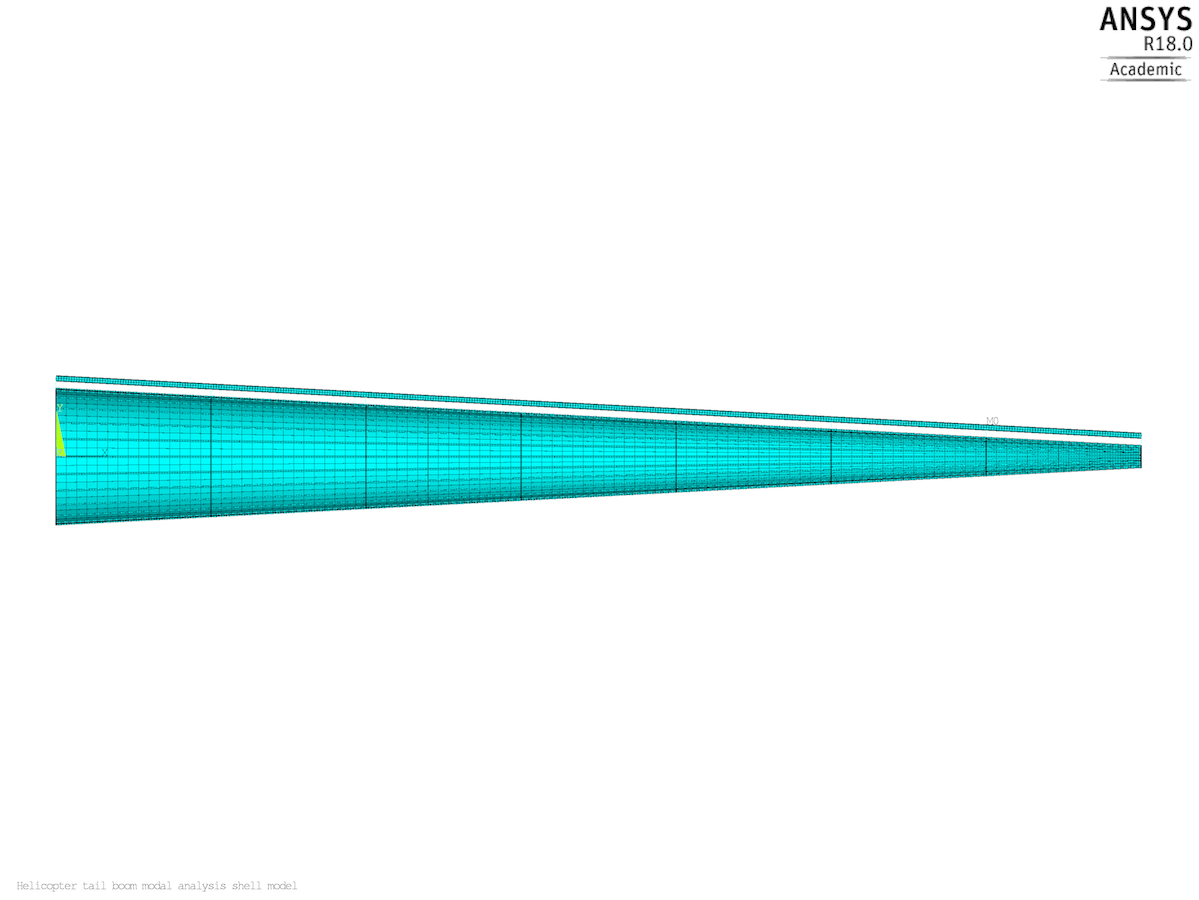
\includegraphics[width=.45\textwidth]{/ShellModelShaft/ShellmodelShaft003}} \quad
\subfloat[][\emph{isometric view}.]
   {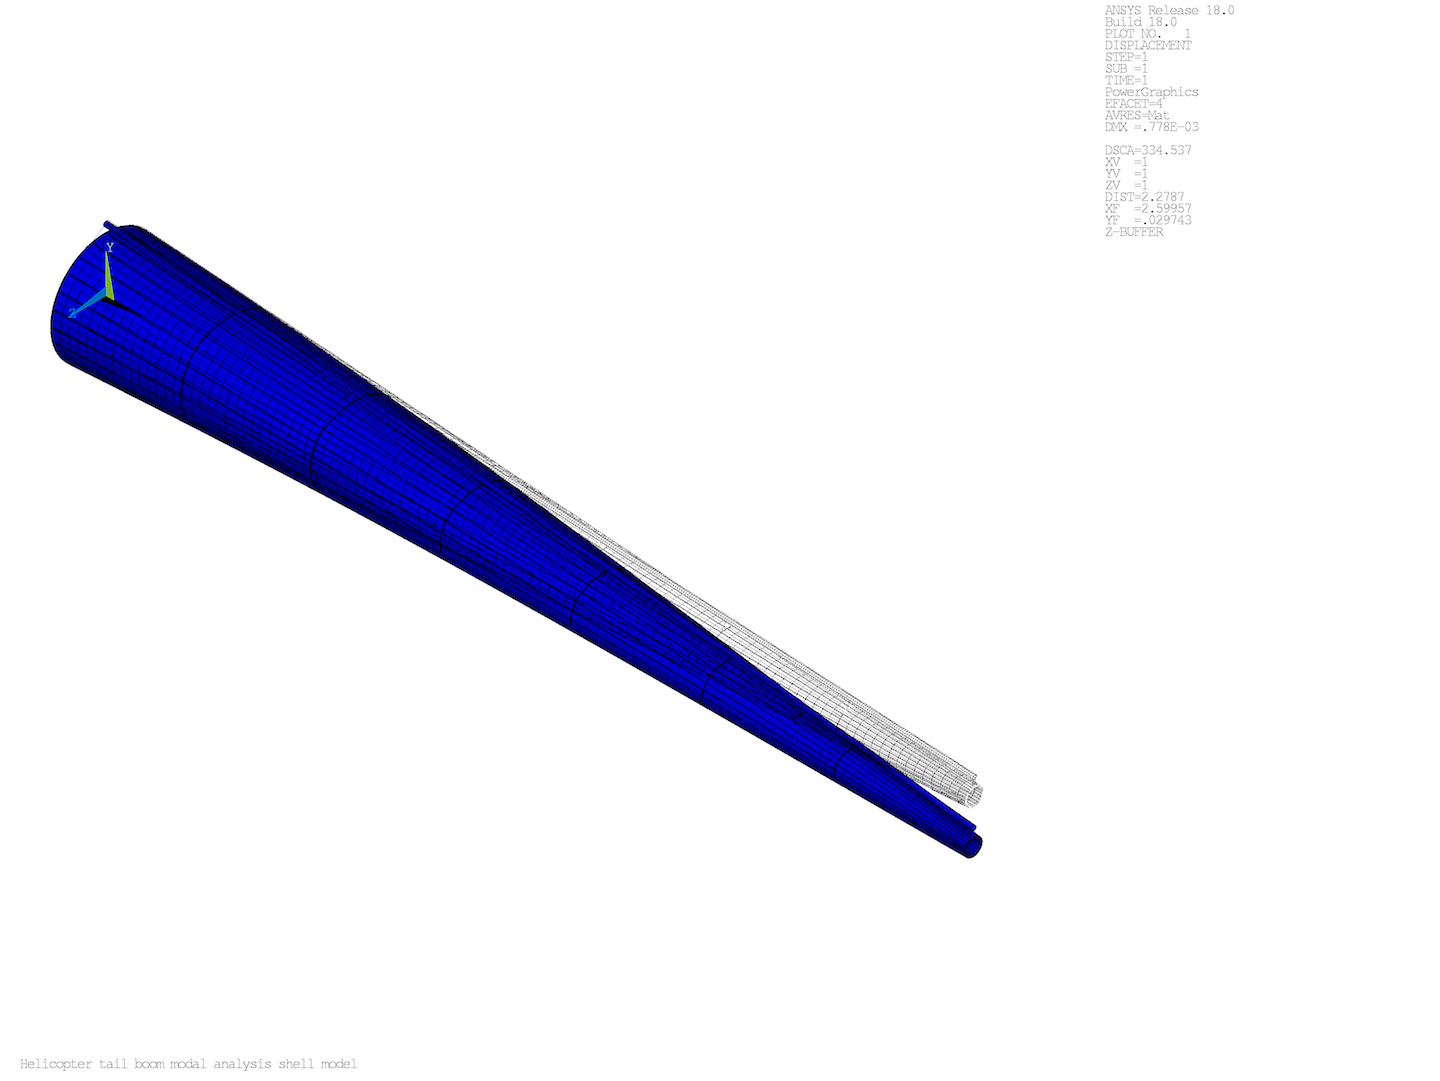
\includegraphics[width=.45\textwidth]{/ShellModelShaft/ShellmodelShaft004}}\\
\caption{Shell model with shaft}
\label{fig:Ansys1MeshShaft}
\end{figure}

\subsection{Simple model with lumped mass}
Starting with the simple model, in this case, the rigid rigid links are added as done to the model with the shaft, but in this case in the connecting terminal part are added the concave mass portions representing the distributed shaft weight. In fact, these are modeled with \textsc{mass21} element type and have the property of having the mass equal to a fraction of the shaft.
Also in this case consider the rotor block as near the tail as modeled in the previous case, the result is visible in fig.\ref{fig:AnsysMeshLumped}.

\begin{figure}[ht]
\centering
\subfloat[][\emph{side view}.]
   {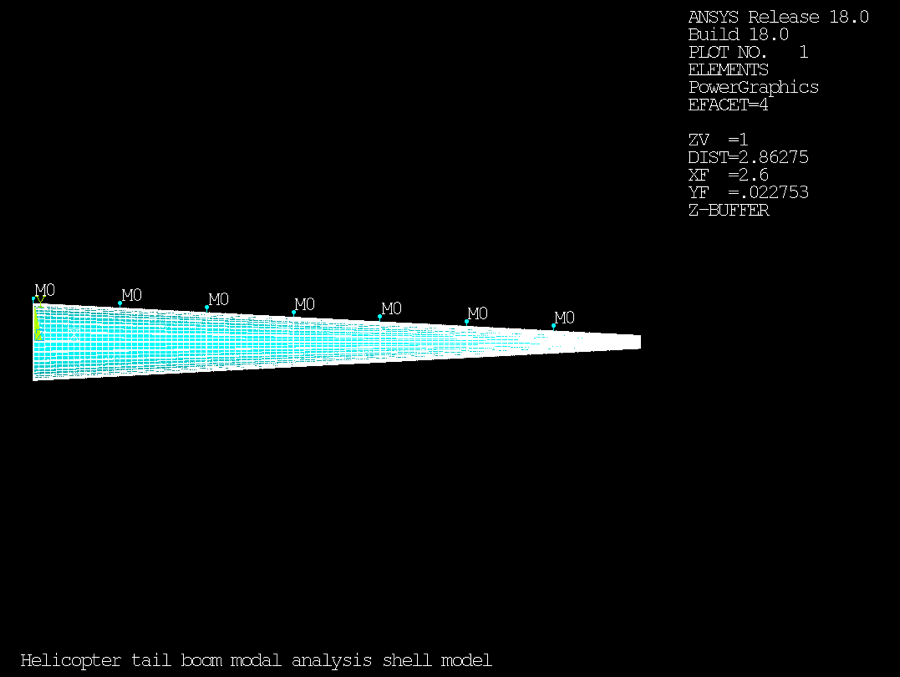
\includegraphics[width=.45\textwidth]{/ShellmodelShaftLumped/ShellmodelShaftLumped003}} \quad
\subfloat[][\emph{isometric view}.]
   {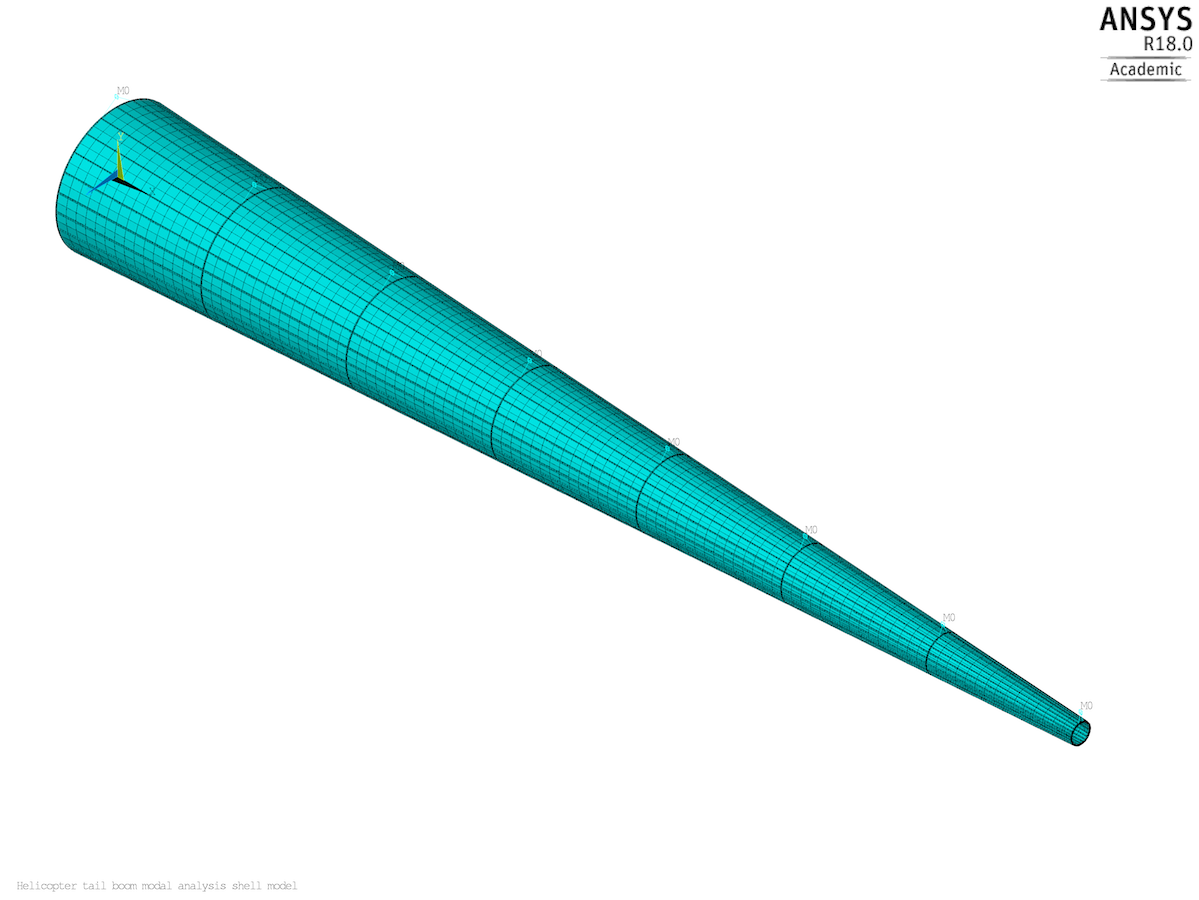
\includegraphics[width=.45\textwidth]{/ShellmodelShaftLumped/ShellmodelShaftLumped004}}\\
\caption{Simple model with lumped mass}
\label{fig:AnsysMeshLumped}
\end{figure}

\newpage

\section{Preliminary analysis}
In the preliminary analysis we have investigated the deformations caused by the proper weight of the structure, in fact this is only subject to gravity acceleration, using an approximate value equal to $9.81\,[m/s^2]$.
Each model has been studied by making it a constraint with a cone at the base of the cone, so it is possible to make a parallelism with a cantilever beam.
In the following, table \ref{tab:RecapStressDeformation}, shows deflection and stress values while you can observe the effects of flexural tension distribution for structures and the effect due to the presence or not of the shaft, osservable in figures \ref{fig:ShellDisplacement}--\ref{fig:ShellNodalSolu}.

\begin{table}[!ht]
\centering
\begin{tabular}{lcc}
	\hline
	Case				& Displacement 	\\
					& $[m]$			\\
	\hline
	Simple model		& 0.00092 		\\
	With shaft		& 0.00346 		\\
	Lumped mass		& 0.00459 		\\
	\hline
\end{tabular}
\caption{Deformation values and stress of the models analyzed}
\label{tab:RecapStressDeformation}
\end{table}

\begin{figure}[ht]
\centering
\subfloat[][\emph{Simple model}.]
   {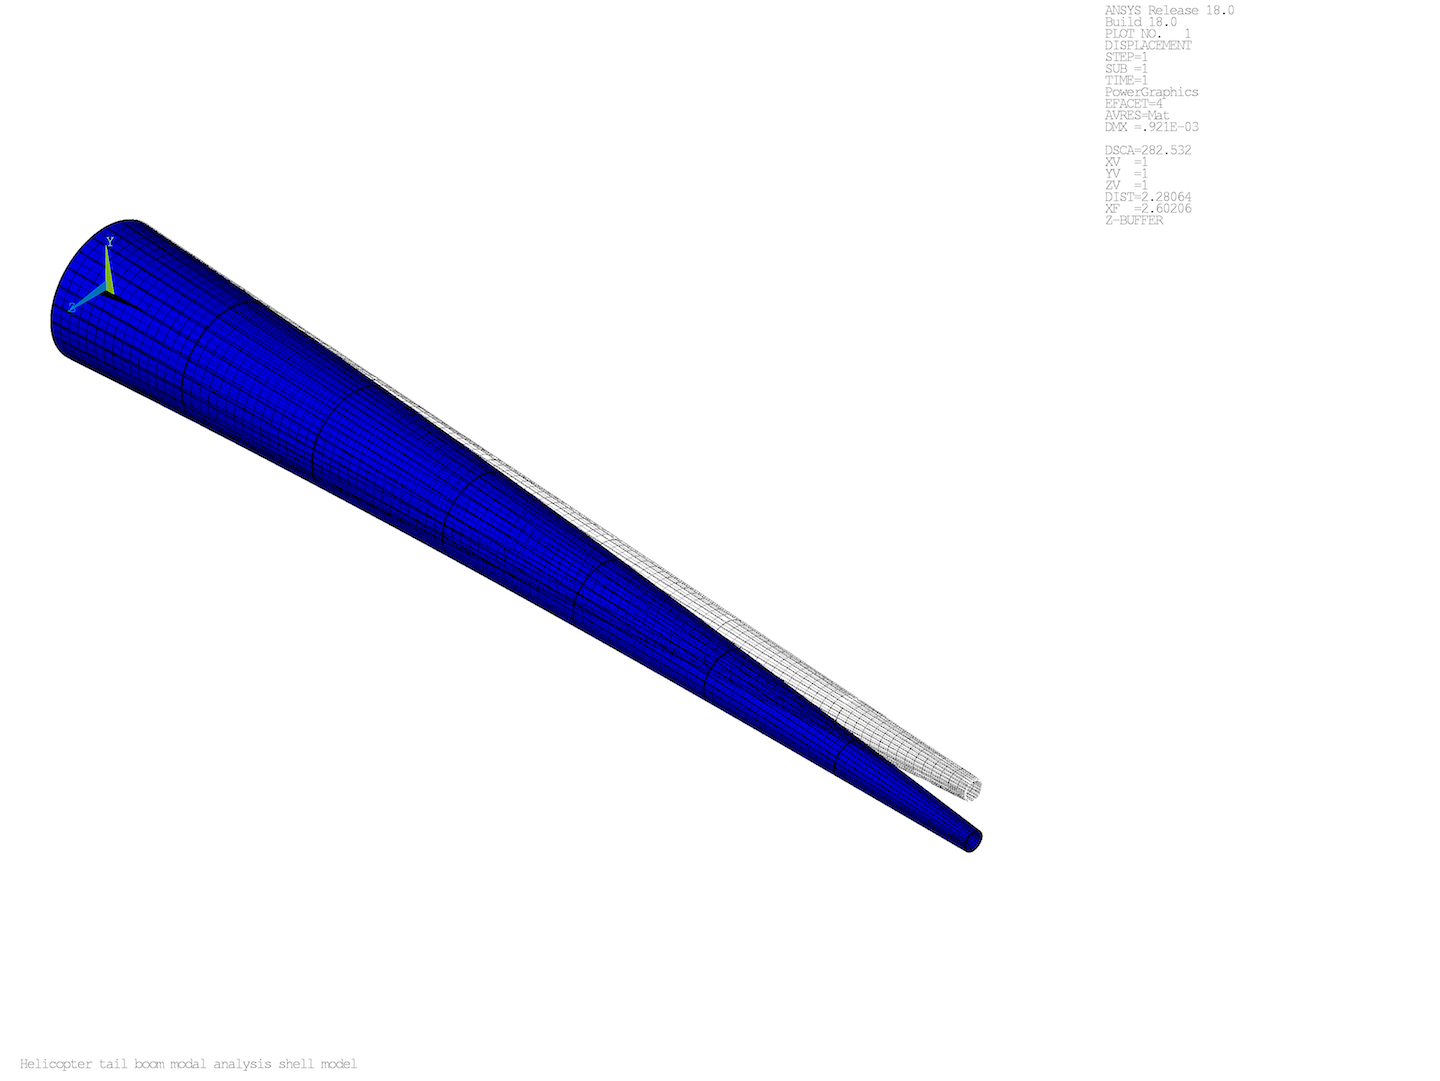
\includegraphics[width=.65\textwidth]{/ShellModel/Shellmodel003}} \,
\end{figure}
\begin{figure}[ht]\ContinuedFloat
\centering
\subfloat[][\emph{Model with Shaft}.]
   {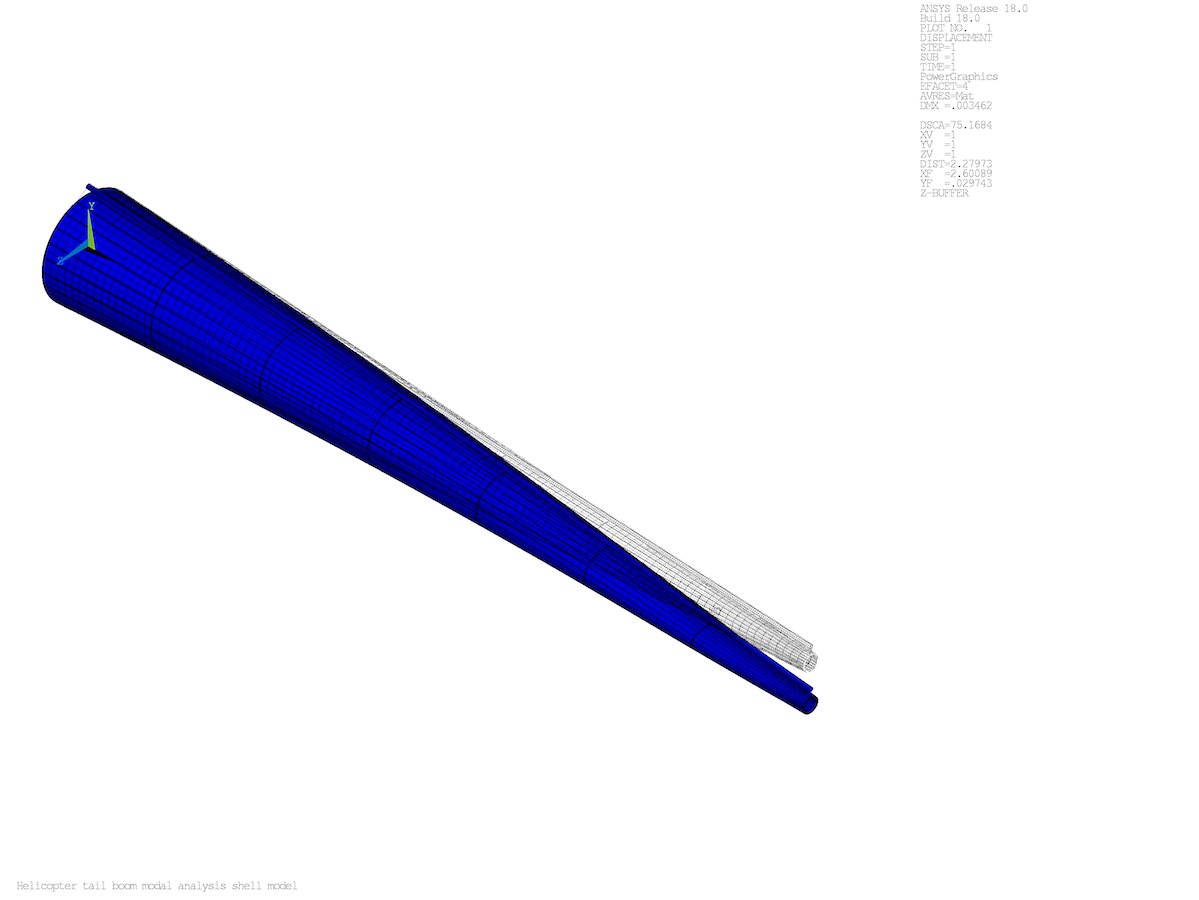
\includegraphics[width=.65\textwidth]{/ShellModelShaft/ShellmodelShaft005}} \\
   \subfloat[][\emph{Model with lumped mass}.]
   {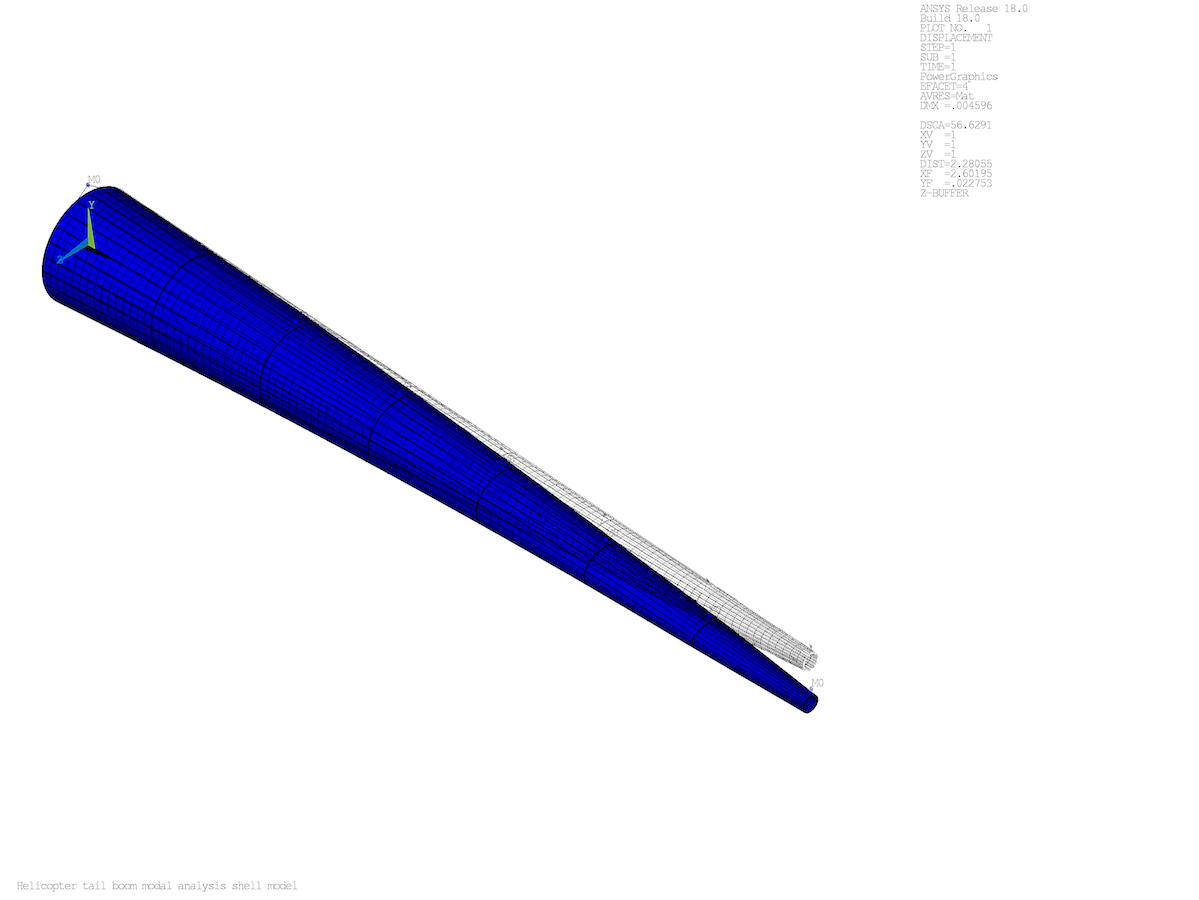
\includegraphics[width=.65\textwidth]{/ShellmodelShaftLumped/ShellmodelShaftLumped005}}\\
\caption{Maximum displacement}
\label{fig:ShellDisplacement}
\end{figure}

\begin{figure}[ht]
\centering
\subfloat[][\emph{Simple model}.]
   {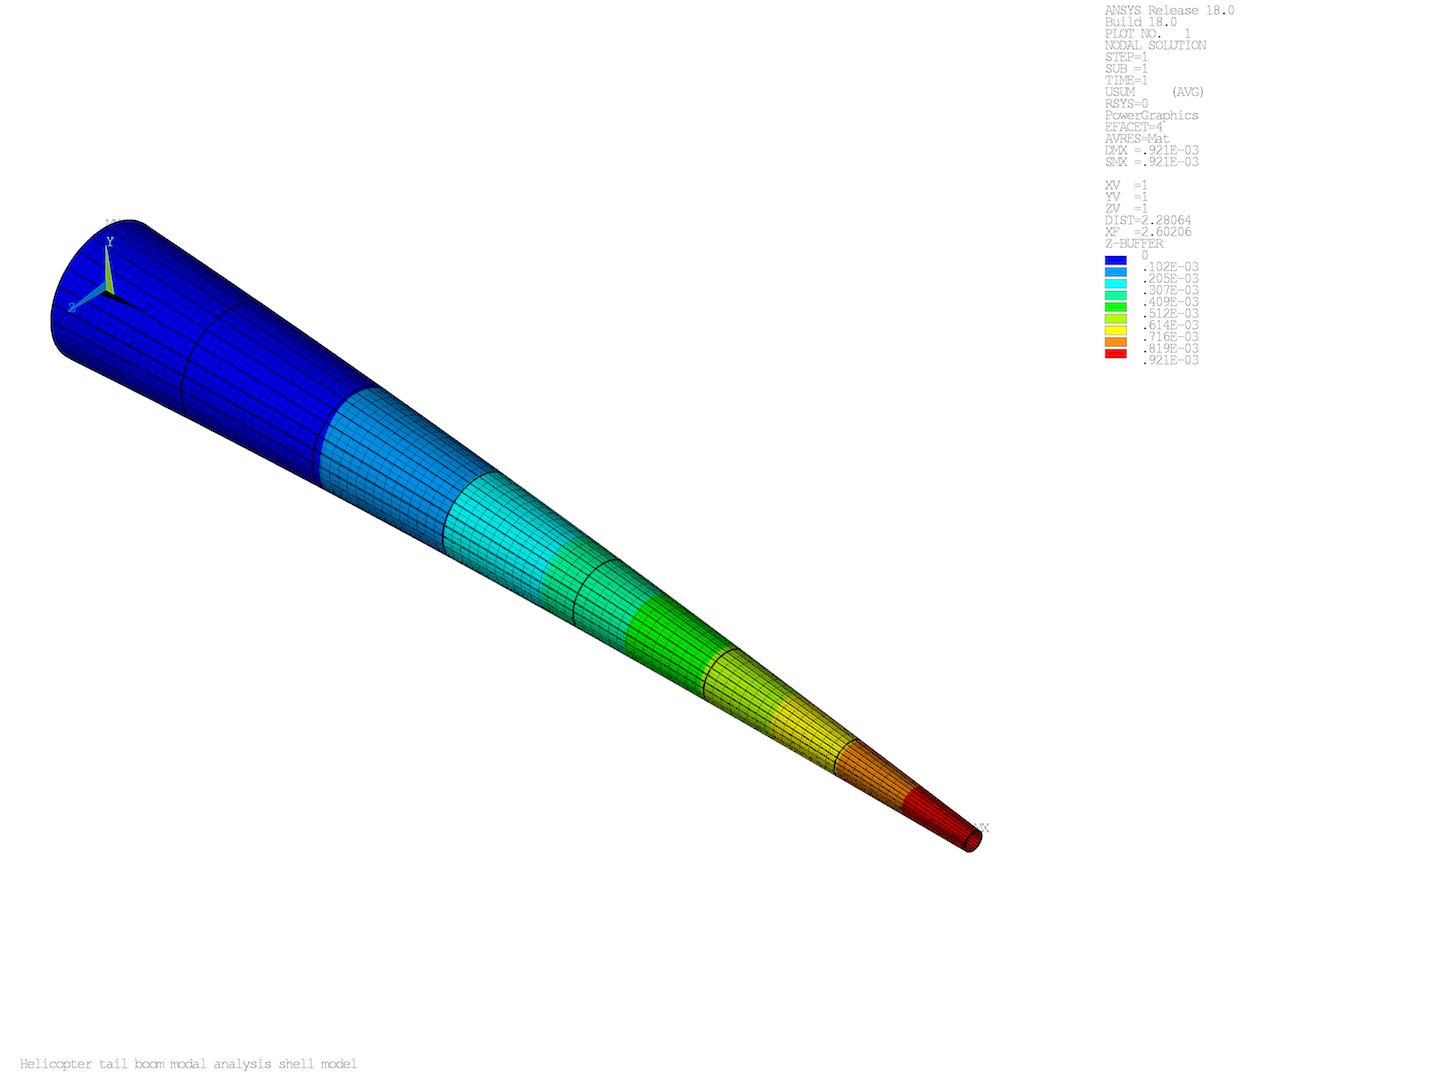
\includegraphics[width=.5\textwidth]{/ShellModel/Shellmodel004}} \,
\subfloat[][\emph{Model with Shaft}.]
   {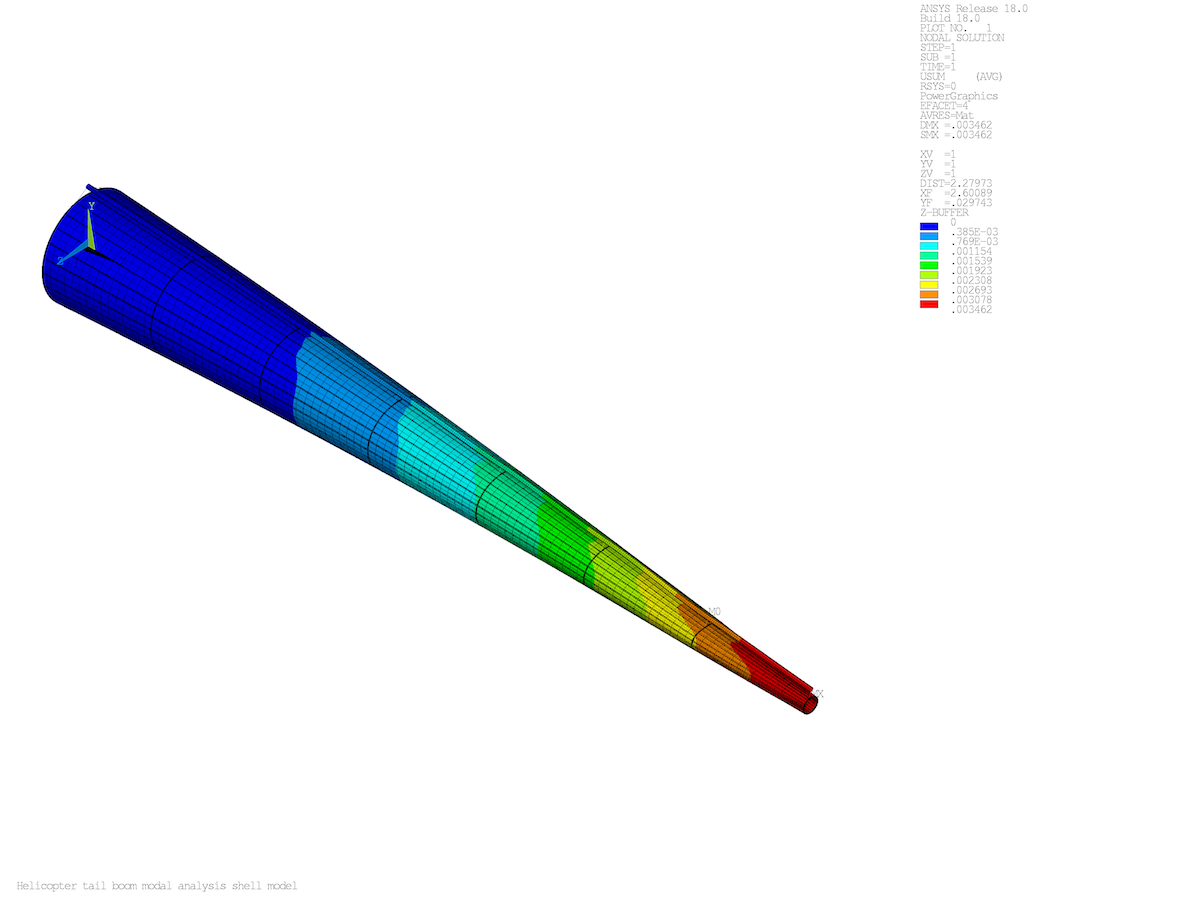
\includegraphics[width=.5\textwidth]{/ShellModelShaft/ShellmodelShaft006}}\\
\subfloat[][\emph{Model with lumped mass}.]
   {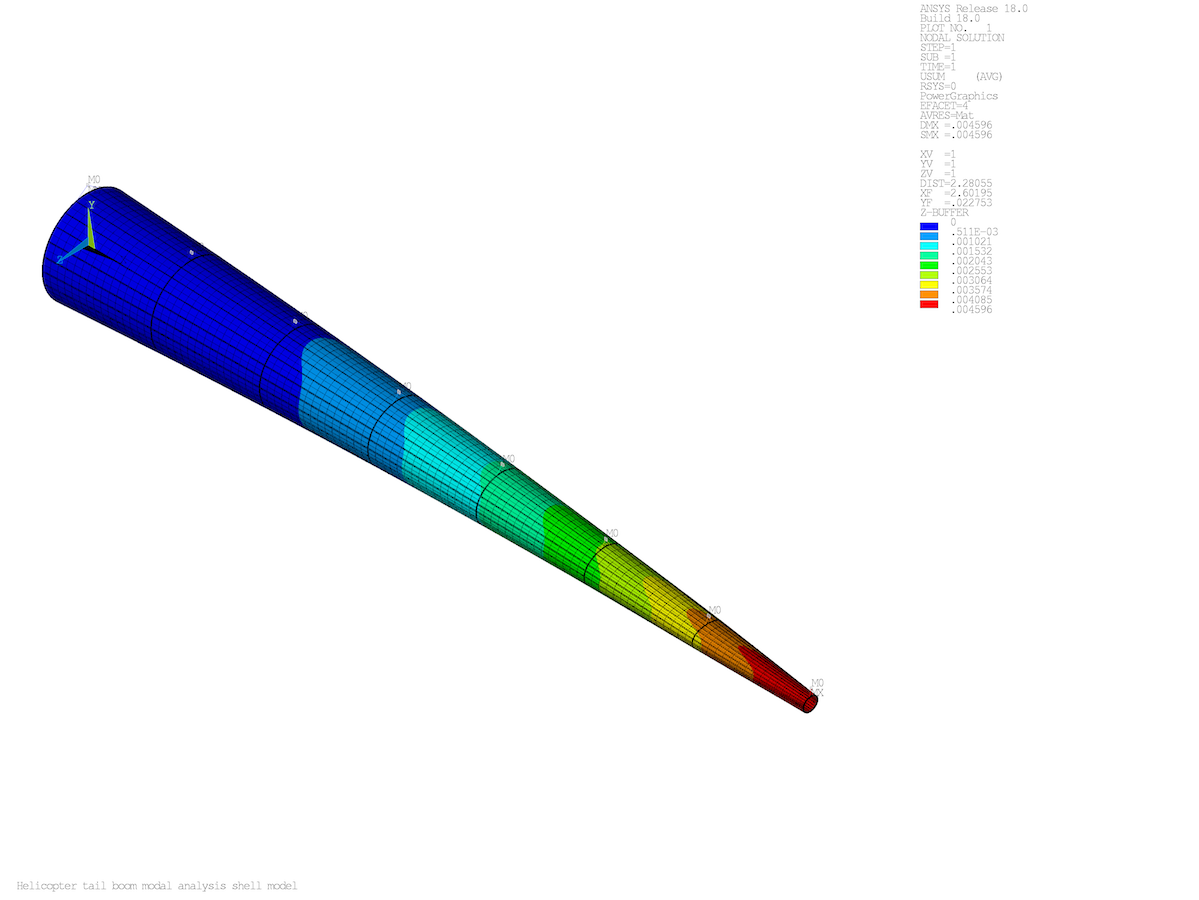
\includegraphics[width=.5\textwidth]{/ShellmodelShaftLumped/ShellmodelShaftLumped006}}\\
\caption{Nodal soluiton}
\label{fig:ShellNodalSolu}
\end{figure}

%\begin{figure}[ht]
%\centering
%\subfloat[][\emph{Simple model}.]
%   {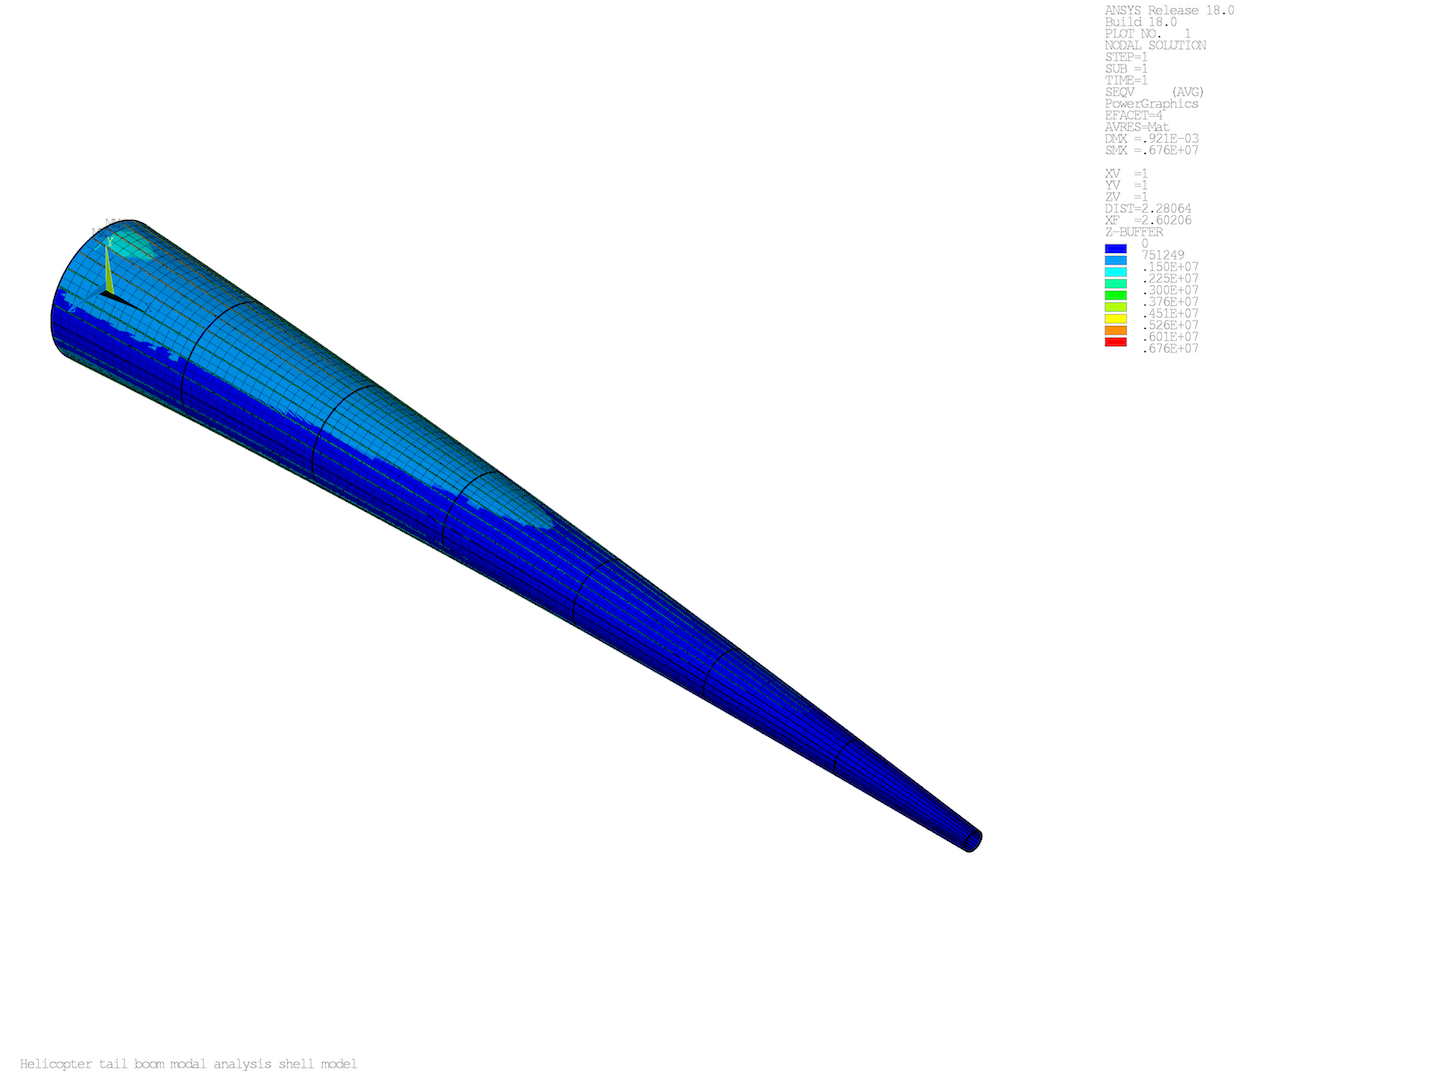
\includegraphics[width=.45\textwidth]{/ShellModel/Shellmodel005}} \quad
%\subfloat[][\emph{Model with Shaft}.]
%   {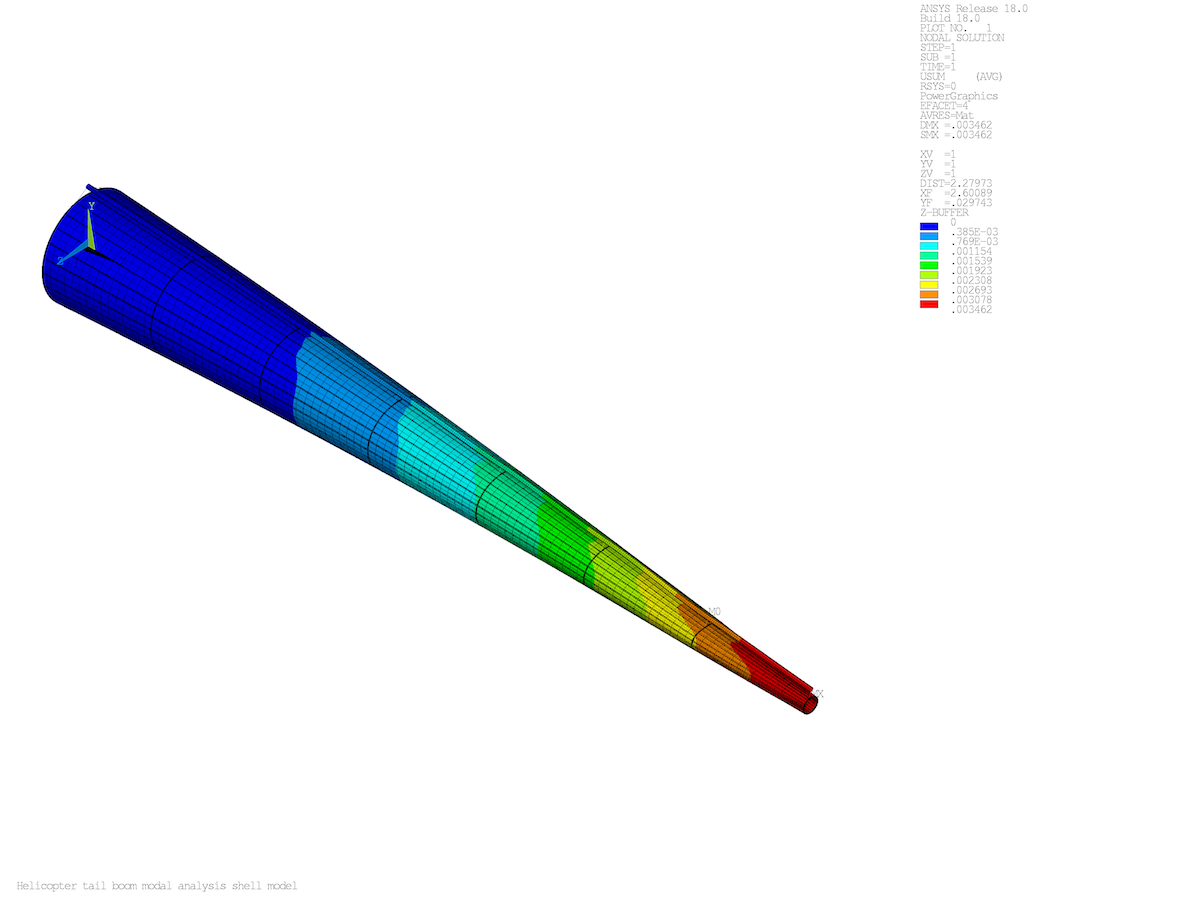
\includegraphics[width=.45\textwidth]{/ShellModelShaft/ShellmodelShaft006}}\\
%\caption{Von Mises equivalent stress}
%\label{fig:ShellVonMises}
%\end{figure}

\section{Modal Analysis}
\begin{table}[h!]
\centering
\pgfplotstableset{
	% global config, for example in the preamble
	% these columns/<colname>/.style={<options>} things define a style
	% which applies to <colname> only.
    every head row/.style={before row=\hline,after row=\hline},
    every last row/.style={after row=\hline},
    display columns/0/.style={column name =Mode, int detect,column type=r},
    display columns/1/.style={column name =Frequence [Hz], column type=r,
	fixed,fixed zerofill,precision=5,set thousands separator={\,}},
    %other style option   
    }
    \pgfplotstabletypeset[col sep=space]{ModalFreq-Shellmodel.txt}
\caption{Natural frequencies for the simple model}
\label{tab:ModalFreq-Shellmodel}
\end{table}

\begin{table}[h!]
\centering
\pgfplotstableset{
	% global config, for example in the preamble
	% these columns/<colname>/.style={<options>} things define a style
	% which applies to <colname> only.
    every head row/.style={before row=\hline,after row=\hline},
    every last row/.style={after row=\hline},
    display columns/0/.style={column name =Mode, int detect,column type=r},
    display columns/1/.style={column name =Frequence [Hz], column type=r,
	fixed,fixed zerofill,precision=5,set thousands separator={\,}},
    %other style option   
    }
    \pgfplotstabletypeset[col sep=space]{ModalFreq-ShellmodelShaft.txt}
\caption{Natural frequencies for the model with shaft}
\label{tab:ModalFreq-ShellmodelShaft}
\end{table}

\begin{table}[h!]
\centering
\pgfplotstableset{
	% global config, for example in the preamble
	% these columns/<colname>/.style={<options>} things define a style
	% which applies to <colname> only.
    every head row/.style={before row=\hline,after row=\hline},
    every last row/.style={after row=\hline},
    display columns/0/.style={column name =Mode, int detect,column type=r},
    display columns/1/.style={column name =Frequence [Hz], column type=r,
	fixed,fixed zerofill,precision=5,set thousands separator={\,}},
    %other style option   
    }
    \pgfplotstabletypeset[col sep=space]{ModalFreq-ShellmodelShaftLumped.txt}
\caption{Natural frequencies for the model with lumped mass}
\label{ModalFreq-ShellmodelShaftLumped}
\end{table}